% Session 9 -- a vacancy as a boundary of zero size, and why that makes it a
% Placement: sec. "Impurities as diagnostics III", after the bulk-boundary paragraph.
% Rendered by figures/blender/s09f04_vacancy.py, labels in figures/overlays/s09f04_vacancy.tex.
\begin{aqmfigure}{fig:s09:vacancy}{Why a single missing atom detects topology. Top, seen from above.
If we cut a large hole into a topologically non-trivial insulator or superconductor, the
bulk-boundary correspondence guarantees gapless modes that run around its edge. Nothing in that
argument depends on the size of the hole, so making it smaller does not remove these modes. A
vacancy is a boundary of zero size, and it binds an in-gap mode. Bottom, schematic spectra. This is
the diagnostic that a clean spectrum cannot give. A trivial and a topological insulator with the
same gap have bulk spectra that look the same, so nothing there distinguishes them (left). If we add
a vacancy, the trivial spectrum stays as it was (middle), and only the topological one develops a
state inside the gap (right). The rule is as direct as it looks. Vacancies produce in-gap modes if
and only if the bulk invariant is non-zero, provided that the vacancy itself respects the symmetry
that protects that invariant.}
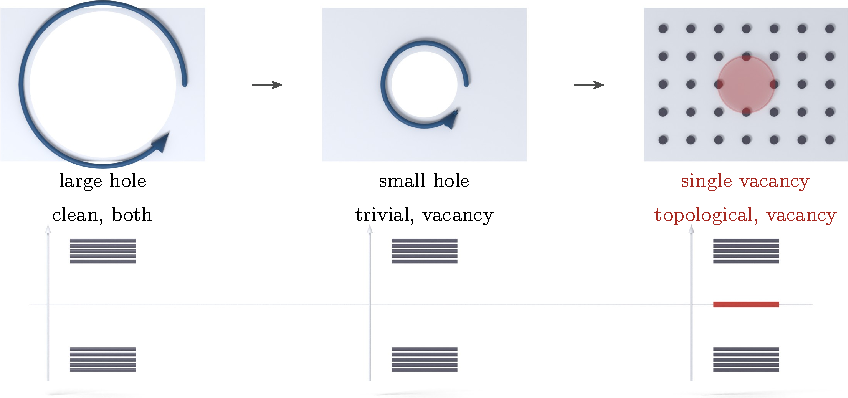
\includegraphics{figures/pdf/s09f04_vacancy.pdf}
\end{aqmfigure}
